%!TEX root =  main.tex
\section{Varying the Exponent}
As seen is the previous sections, the change between squaring the residuals in the original $F$-test to taking their absolute value with the $F_1$-statistic improved power significantly in the differentially-private case. It isn't clear that switching the exponent from 2 to 1 is optimal. While the edge case of raising the differences to the $0^{\text{th}}$ power is clearly not optimal, some value between 0 and 2 other than 1 could be. In order to determine which exponent is in fact optimal, we first generalize the notion of an $F$-test even further. 

\subsection{Equations and Sensitivities}
Define the \sqa and \sqe, which are equivalent to the \ssa and \sse, except the summand is raised to the $q^{\text{th}}$ exponent. Note that taking the absolute value of the summand is additionally necessary as it may not be positive. 
%%%
\begin{definition}[$F_q$] \label{def:Fq} 
Given a database \x with \k groups and \dbsize total entries, define \sqa and \sqe as follows:
%
\begin{equation*}
\sqa = \sum_{j=1}^k n_j \left\vert \overline{y}_j - \overline{y} \right\vert^q
\end{equation*}
%
\begin{equation*}
\sqe = \sum_{i=1}^N \left\vert y_i - \overline{y}_{c_i} \right\vert^q
\end{equation*}
%
Then, $F_q$ is defined as
%
\begin{equation*}
F_q = \frac{\sqa/(\k-1)}{\sqe/(\dbsize-\k)}
\end{equation*}
%
\end{definition}
%%%
To develop a differentially private $F_q$-test, we first bound the sensitivity of the \sqa and \sqe.
%%%
\begin{theorem}[\sqe Sensitivity] \label{thm:SQEsens} 
The sensitivity of \sqe is bounded above by
\begin{equation*}
2\bigg(\frac{\dbsize}{2}\bigg)^{(1-q)} + 1
\end{equation*}
when $q \in (0,1)$ and
\begin{equation*}
\dbsize - \dbsize\bigg(1-\frac{2}{\dbsize}\bigg)^q +1 
\end{equation*}
when $q\geq 1$. Note that both give an upper bound of 3 when $q=1$.
\end{theorem}
\begin{proof}
As in the previous proofs of the sensitivity of \se and \sa, suppose neighboring databases \x and \xprime differ by some row $r$, with $c_r = a$ in \x and $c_r = b$ in \xprime. Rewrite the \sqe as a sum that indexes over group size and entries within each group.
%
$$\sqe = \sum_{j=1}^k \sum_{i \in C_j} \left\vert  y_i - \overline{y}_{c_i} \right\vert^q.$$
%
Let $t_i =  \left\vert y_{i} - \overline{y}_{c_i} \right\vert ^q$ for any entry $i$.  Note that unless $c_i = a,b$, then $t_i$ will not change between databases \x and \xprime, as the group means of the other groups are not altered. Thus, unless $i$ is in group $a$ or $b$, $t_i$ will contribute nothing to the overall sensitivity of the \sqe. For notational ease, let $z = y_i-\overline{y}_{c_i}$ and parametrize $t_i$ as a function of $z$. We now bound the sensitivity by maximizing $t_i$ when $c_i = a,b$.

\noindent\textbf{Case 1:}
When $q$ is less than $1$, $t_i(z)$ is a concave function with minimum at $z=0$ that is symmetric about the y-axis and which monotonically increases for positive $z$. So, the worst case sensitivity is between $z = 0$ and $z = \frac{1}{n_i}$,\igh{This is the first time this argument is used in the paper so should maybe add a clarifying statement.} and hence
%
\begin{align*}
\Delta t_{i} &\le \left\vert t_i(0) - t_i(1/n_i) \right\vert \\
	&= (1/n_i)^q.
\end{align*}
%
Let $\alpha$ be the upper bound of $\Delta t_i$ when $i \in a, i \ne r$, and let $\beta$ be the upper bound of $\Delta t_i$ when $i \in b, i \ne r$. I.e. $\alpha = (1/n_a)^q$ and $\beta = (1/n_b)^q$.  Then, the total sensitivity of the SQE for $q<1$ is
%
\begin{align*}
\Delta \sqe &\le \left\vert n_a \alpha + n_b \beta + 1 \right\vert \\
	&\le n_a^{1-q} + n_b^{1-q} + 1.
\end{align*}

Recall that the group sizes are not public information, but that the total database size is. So, the question is how much the distribution of the total database between the groups can affect the total sensitivity.\igh{Rephrase} Since $n_i$ is a positive integer and $q<1$, $n_i^{1-q}$ increases for a given $q$ as $n_i$ increases. So, the worst-case sensitivity will occur when as much of the total database is in groups $a$ and $b$ as possible. Write $n_b = N-n_a$. Then,

$$n_a^{1-q} + (N-n_a)^{1-q}$$

\noindent is a downward facing parabola-like function with maximum value when the $n_a = \frac{1}{2}(N-1)$.\igh{Wait where's the -1 coming from...} So, the sensitivity of the \sqe is bounded above by

$$\Delta \sqe \le 2\left(\frac{N}{2}\right)^{1-q} + 1.$$

\noindent\textbf{Case 2:}
When $q$ is greater than $1$, $t_{i}$ is a convex function with maximum at $z=1$, symmetric about the $y$-axis, and monotonically increasing for positive $z$. So, the worst case sensitivity is between $z=1$ and $z=1-1/n_i$, and hence 
%
\begin{align*}
\Delta t_{ij} &\le \left\vert t_{i}(1) - t_{i}(1-1/n_i) \right\vert \\
	&= 1 - (1-1/n_i)^q.
\end{align*}
%
So, 
%
$$ \Delta\sqe \le n_a(1-(1-1/n_a)^q) + n_b(1-(1-1/n_b)^q) + 1.$$

Then, the sensitivity will be maximized when as much of the database is distributed between $n_a$ and $n_b$ as possible. To determine what the worst case allocation is, let 
$$f = n_a(1-(1-1/n_a)^q) + (N-n_a)(1-(1-1/(N-n_a))^q) + 1,$$
i.e. $f$ is an expression for the upper bound of $\Delta\sqe$ with $n_b$ replaced by $N-n_a$ to maximize sensitivity. Then, we can maximize $f$ in terms of $n_a$:
$$ \frac{\partial \Delta f}{\partial n_a} =  -\frac{1-q}{(N - n_a)^q} + \frac{1-q}{n_a^q}$$
has a critical point at $n_a = N/2$, and 
$$ \frac{\partial \Delta^2 f}{\partial n_a^2} = - \frac{(1-q)q}{(N-n_a)^{-1-q}} - \frac{(1-q)q}{n_a^{-1-q}}$$
is always negative. So, $f$ is concave down and $n_a = N/2$ is a global maximum. Hence, the worst case sensitivity occurs when the database is distributed equally between groups $a$ and $b$, i.e. 

$$ \Delta\sqe \le N \left( 1- \left(1-\frac{2}{N}\right)^q \right) + 1.$$
\end{proof}
\begin{theorem}[\sqa Sensitivity]\label{thm:SQAsens} The sensitivity of \sqa is bounded above by 
\begin{equation*}
\dbsize\bigg(\frac{3}{\dbsize}\bigg)^q + 1
\end{equation*}
when $q \in (0,1)$ and
\begin{equation*}
\dbsize-\dbsize\bigg(1-\frac{3}{\dbsize}\bigg)^q + 1
\end{equation*}
when $q \geq 1$. Note that both give an upper bound of 4 when $q = 1$.
\end{theorem}

\begin{proof}
Let $s_{i} =  \left\vert \bar{y}_{i} - \grand \right\vert ^q$ for any group $i$. I.e., $s_{i}$ is the (unweighted) term in the calculation of the \sqa that corresponds to group $i$. Note that as the grand mean changes between databases $\x$ and $\xprime$ in addition to the group mean, all groups, not just groups $a$ and $b$, will contribute to the sensitivity of the \sqa. Recall that the sensitivity of the grand mean is $1/N$, while the sensitivity of the group mean for groups $a$ and $b$ are $1/n_a$ and $1/n_b$ respectively. \\

\noindent\textbf{Case 1:} When $q$ is less than $1$, $s_i$ is a concave function with minimum at $x=0$, symmetric about the $y$-axis, and monotonically increasing for positive $x$. So, the worst case sensitivity of $\Delta s_i$ for $i \ne a,b$ is between $x=0$ and $x=1/N$, and the worst case sensitivity of $\Delta s_i$ for $i = a,b$ is between $x=0$ and $x=1/n_i + 1/N$. Then, the total sensitivity of the \sqa for $q<1$ is
%
$$ \Delta\sqa \le \left\vert (N-n_a-n_b-1)(1/N)^q + n_a(1/N + 1/n_a)^q + n_b(1/N + 1/n_b)^q + 1\right\vert. $$
%
The addition of the $1$ comes from the fact that our data point that switches between groups contributes $\vert \bar{y_a} + \grand \vert$ to the calculation of the \sqa in database \x, and contributes $\vert \bar{y_b} + \grand \vert$ to the calculation of the \sqa in database \xprime; the difference between these two terms is bounded above by 1. Note that since $q<1$, $(1/x)^q > 1/x$. Hence, $(1/N + 1/n_a)^q > (1/N)^q$ and thus the worst-case sensitivity occurs when all of $N$ is allocated to groups $a$ and $b$. I.e,
%
$$ \Delta\sqa \le n_a(1/N + 1/n_a)^q + (N-n_a)(1/N + 1/(N-n_a))^q. $$
Then, as in the proof of the \sqe's sensitivity, to determine the worst-case sensitivity in terms of $N$, let 
$$g = n_a(1/N + 1/n_a)^q + (N-n_a)(1/N + 1/(N-n_a))^q $$
and maximize this expression in terms of $n_a$:
$$ \frac{\partial g}{\partial n_a} = -\left(\frac{1}{N} + \frac{1}{N-n_a}\right)^q + \left(\frac{1}{N} + \frac{1}{n_a}\right)^q + \frac{(\frac{1}{N} + \frac{1}{N-n_a})^{q-1})q}{N-n_a} - \frac{(\frac{1}{N} + \frac{1}{n_a})^{q-1}q}{n_a}$$
is a symmetric expression between $N$ and $N-n_a$. So, there must be a critical point at $n_a = N/2$. Then, since
\begin{align*}
\frac{\partial^2 g}{\partial n_a^2} &= N^2(q-1)q \left( \frac{(\frac{1}{N} + \frac{1}{N-n_a})^q}{(N-n_a)(-2N+n_a)^2} + \frac{\left(\frac{1}{N} + \frac{1}{n_a}\right)^q}{n_a(N+n_a)^2}\right) \\
	&\le 0,
\end{align*}
since $N>n_a$ and $q<1$. So, $n_a = N/2$ is a global maxima, and hence
%
$$\Delta\sqa \le N \left( \frac{3}{N} \right)^q.$$
\noindent\textbf{Case 2:} When $q$ is greater than $1$, $s_i$ is a convex function with minimum at $x=0$, symmetric about the $y$-axis, and monotonically increasing for positive $x$. So, the worst case sensitivity of $\Delta s_i$ for $i \ne a,b$ is between $x= 1$ and $x=1-1/N$, and the worst-case sensitivity of $\Delta s_i$ for $i=a,b$ is between $x = 1 - 1/N - 1/n_i$ Then, the total sensitivity of the \spa for $q<1$ is
%
\begin{align*}
\Delta\sqa &\le \vert (N-n_a-n_b)(1-(1-1/N)^q) + n_a(1-(1-1/N-1/n_a)^q) \\
	& \hspace{1cm} + n_b(1-(1-1/N-1/n_b)^q + 1\vert \\
	&= (N-n_a-n_b)(1-(1-1/N)^q) + n_a(1-(1-1/N-1/n_a)^q) \\
	& \hspace{1cm} + n_b(1-(1-1/N-1/n_b)^q + 1. 
\end{align*}
%
Note that 
%
\begin{align*}
1-1/N-1/n_b &< 1-1/N \\
\Rightarrow (1-1/N-1/n_b)^q &< (1-1/N)^q \\
\Rightarrow 1 - (1-1/N-1/n_b)^q &> 1- (1-1/N)^q.
\end{align*}
Thus, $\Delta\sqa$ is maximized when $N$ is maximally allocated to groups $a$ and $b$. As in the proof for $q<1$, this occurs when $n_a = N/2 = n_b$. Then, 
$$\Delta\sqa < N \left( 1 - \left( 1 - \frac{3}{N}\right)^q \right)$$
\end{proof}

\subsection{Power Analysis}
\ar{You can start by referencing the previous Power Analysis section (Section~\ref{subsec:power-analysis}).}  We ran many different exponents on various effect sizes and epsilons, and $q=1$ is the optimal choice. \ar{I'm assuming this will be fleshed out once the figures are in?  This seems to be THE major result, at least empirically.}
\begin{figure}
\centering
\includegraphics[width=\linewidth]{figure6F_standardeffect.png}
%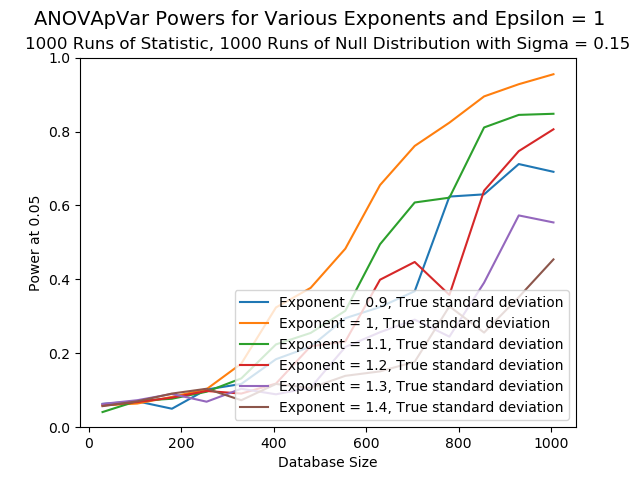
\includegraphics[width=0.8\textwidth,natwidth=610,natheight=642]{Placeholder_manyExponents.png}
\caption{Power is experimentally maximized when $q = 1$.}
\end{figure}

